%%%%%%%%%%%%%%%%%%%%%%%%%%%%%%%%%%%%%%%%%%%%%%%%%%%
%
%  New template code for TAMU Theses and Dissertations starting Fall 2012.
%  For more info about this template or the
%  TAMU LaTeX User's Group, see http://www.howdy.me/.
%
%  Author: Wendy Lynn Turner
%	 Version 1.0
%  Last updated 8/5/2012
%
%%%%%%%%%%%%%%%%%%%%%%%%%%%%%%%%%%%%%%%%%%%%%%%%%%%
%%%%%%%%%%%%%%%%%%%%%%%%%%%%%%%%%%%%%%%%%%%%%%%%%%%%%%%%%%%%%%%%%%%%%%
%%                           SECTION III
%%%%%%%%%%%%%%%%%%%%%%%%%%%%%%%%%%%%%%%%%%%%%%%%%%%%%%%%%%%%%%%%%%%%%



\chapter{\uppercase{Results and Conclusions}}

Each language had it's own advantages and disadvantages to the ray tracing process.  These were futher accentuated by the speed tests conducted for each Milestone.  The results for each speed test were to be as expected from common knownledge of each language, and from more rigourous tests conducted by other computer scientists.  Python was the slowest by far, with Processing holding the middle ground and C++ being the fastest.  Surprisingly however, the speed difference between Process and C++ is less than what might have been expected, since C++ is compiled before running the test and Processing's speed test is considered with the processing ``play'' button.  

\section{Conclusions}
Each language will be discussed with it's pro's and con's and at the end of this section a reccomendation will be made as to the most suitable language that might maximize focus on the implementation theory rather than the implementation process of writing code syntax.  It can be established as a baseline for all languages however that you MUST learn a certain baseline of scripting and coding concepts. Language syntax and compilation processes cannot be avoided.  

\subsection{C++}
C++ is the fastest processor of all the languages tested.  This allowed for quicker iterations and more creative freedom with the final images because of the quick process speed.  
%%%%%%%%%%%%%%%%%%%%%%%%%%%%%%%%%%%%%%%%%%%%%%%%%%%%%%
\begin{figure}[H]
\centering
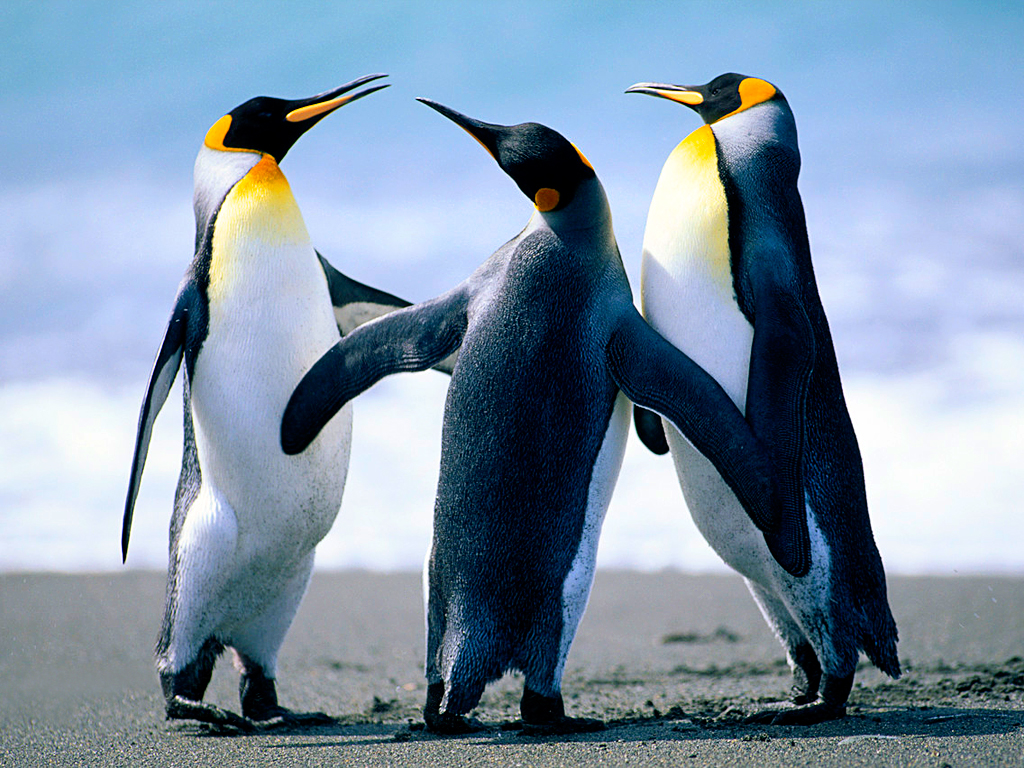
\includegraphics[scale=.50]{figures/Penguins.jpg}
\caption{TAMU figure}
\label{fig:tamu-fig3}
\end{figure}
%%%%%%%%%%%%%%%%%%%%%%%%%%%%%%%%%%%%%%%%%%%%%%%%%%%%%%
\section{Another Section}

Text between the figures.  Text between the figures. Text between the figures. Text between the figures.  Text between the figures. Text between the figures. Text between the figures.  Text between the figures. Text between the figures. Text between the figures.  Text between the figures. Text between the figures.
%%%%%%%%%%%%%%%%%%%%%%%%%%%%%%%%%%%%%%%%%%%%%%%%%%%%%%%
%\begin{figure}[H]
%\centering
%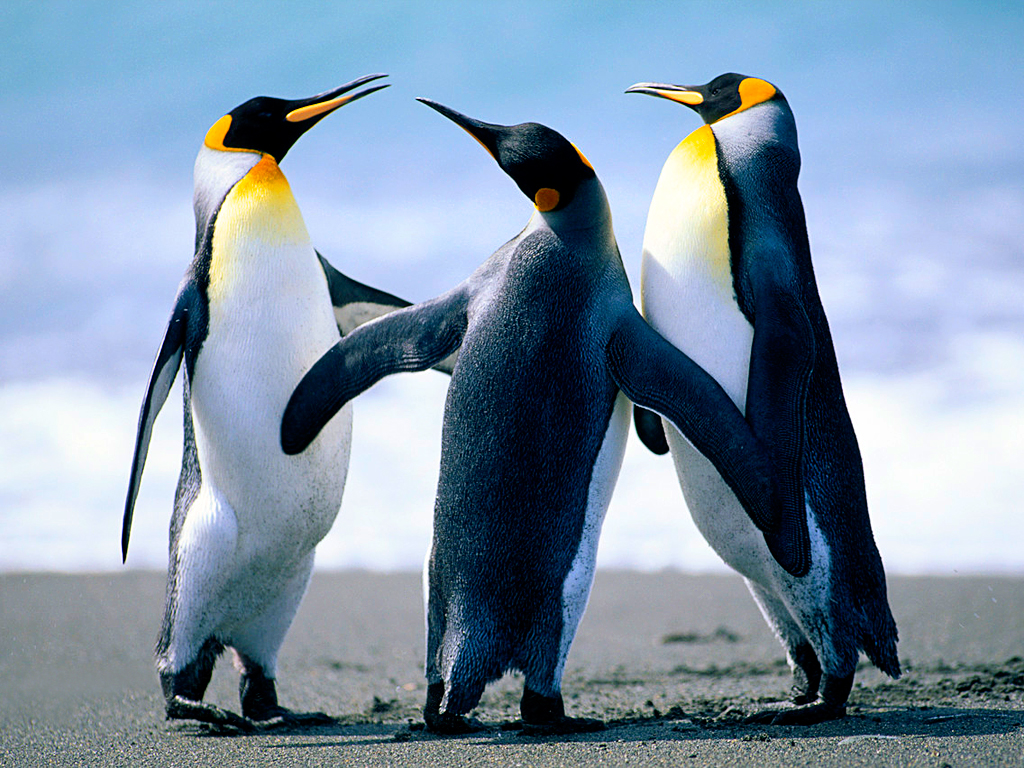
\includegraphics[scale=.50]{figures/Penguins.jpg}
%\caption{Another TAMU figure}
%\label{fig:tamu-fig4}
%\end{figure}
%%%%%%%%%%%%%%%%%%%%%%%%%%%%%%%%%%%%%%%%%%%%%%%%%%%%%%%

\subsection{Subsection}

%%%%%%%%%%%%%%%%%%%%%%%%%%%%%%%%%%%%%%%%%%%%%%%%%%%%%%%
%\begin{figure}[H]
%\centering
%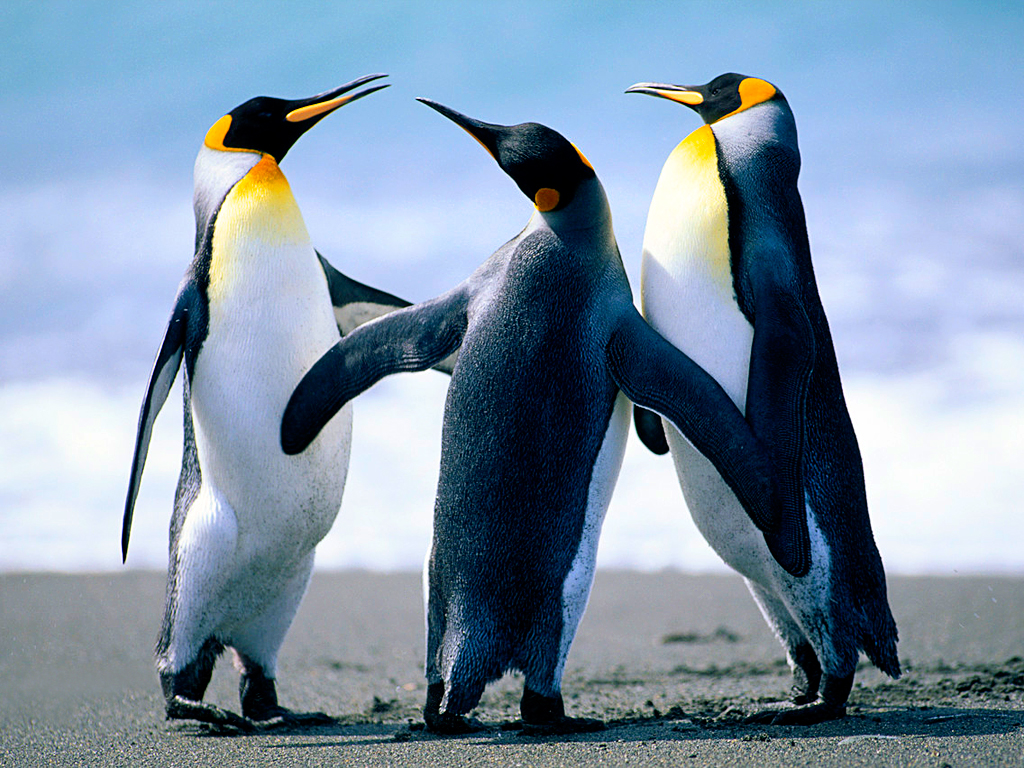
\includegraphics[scale=.50]{figures/Penguins.jpg}
%\caption{Another TAMU figure}
%\label{fig:tamu-fig4-2}
%\end{figure}
%%%%%%%%%%%%%%%%%%%%%%%%%%%%%%%%%%%%%%%%%%%%%%%%%%%%%%%
\subsection{Subsection}

A table example is going to follow.

\begin{table}[H]
\centering
\caption{This is a table template}
\begin{tabular}{|l|c|c|c|c|c|}
\hline
Product & 1 & 2 & 3 & 4 & 5\\
\hline
Price & 124.- & 136.- & 85.- & 156.- & 23.-\\
Guarantee [years] & 1 & 2 & - & 3 & 1\\
Rating & 89\% & 84\% & 51\% & & 45\%\\
\hline
\hline
Recommended & yes & yes & no & no & no\\
\hline
\end{tabular}
\label{tab:template2}
\end{table}
\section{Another Section} 